\subsection{A-Scan\label{sec:AScan}}
\subsection{B-Scan}
Zur einfacheren Beschreibung des Vorgehens wird nun definiert, dass die obere Kante in Abbildung \ref{fig:acrylblock} \emph{oben} sein soll und die in der Abbildung untere Kante \emph{unten}. \\
Es werden zwei B-Scans aufgenommen, einmal mit \emph{oben} oben und einmal mit \emph{unten} oben. Sie sind in Abbildung \ref{fig:BScan} dargestellt. Die Skala jeweils rechts kennzeichnet die Stärke des reflektierten Signals. Mit Hilfe des Bildbearbeitungsprogrammes \emph{gimp} und seiner \emph{Measure}-Funktion werden die Laufzeiten der Signale in den Graphiken gemessen. Genauer: Die Laufzeit des Signals von \emph{oben} bis zum jeweiligen Loch wird aus \ref{fig:oben} und die Laufzeit von \emph{unten} wird aus \ref{fig:unten} abgelesen. Abbildung \ref{fig:Schema} zeigt welcher Abstand dafür genau gewählt wird.
\begin{figure}[h!]
	\centering
	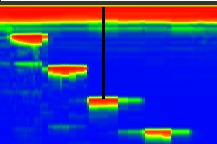
\includegraphics[width=0.35\textwidth]{Schema.png}
	\caption{Die senkrechte schwarze Linie kennzeichnet welcher Abstand im B-Scan zur Bestimmung der Laufzeit des Signals verwendet wird.}
	\label{fig:Schema}
\end{figure} \\
\todo[color = red, inline]{Hier dachte ich: OK, bei rot ist immer irgendwie Luft, bzw. ganz oben ist der rote Balken halt der Übergang zwischen Sonde und Glas. Also messe ich von der Unterkante des roten Balkens (weil da ja das Glas erst losgeht) bis zur Oberkante des jeweiligen Lochs. Dann sind die Werte aber viel zu klein. Von der Oberkante weg passts ganz gut. Kannst du das erklären?}
\todo{Ja, ich weiß, die Scans sind sehr klein, aber für ein Protokoll ist das sonst zu viel Tintenverschwendung.}
\begin{figure}[h!]
	\centering
	\begin{subfigure}{.45\textwidth}
		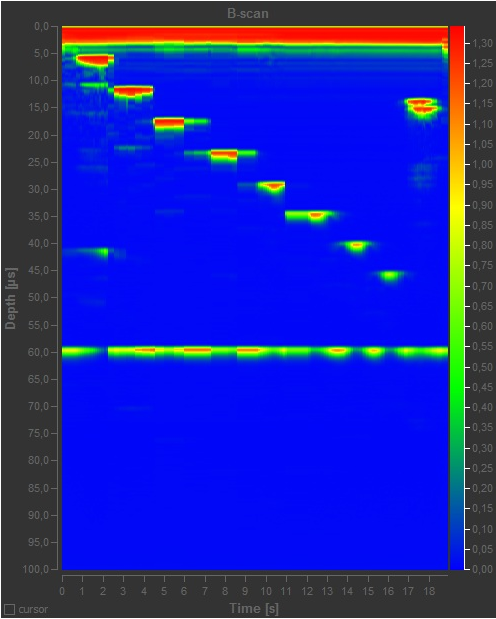
\includegraphics[width=\textwidth]{oben.png}
		\caption{von \emph{oben}}
		\label{fig:oben}
	\end{subfigure}
	\begin{subfigure}{.45\textwidth}
		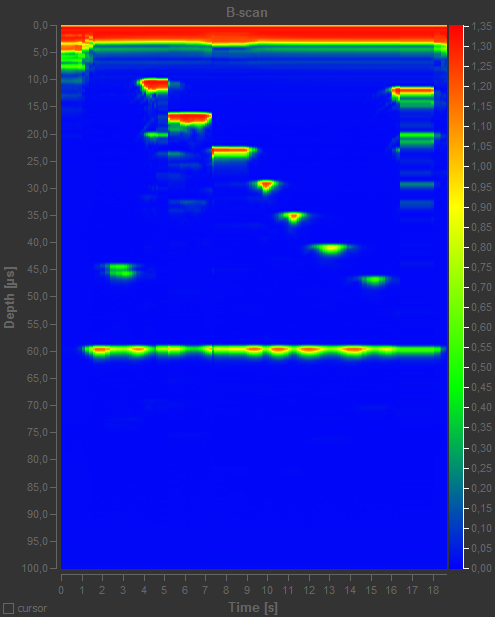
\includegraphics[width=\textwidth]{unten.png}
		\caption{von \emph{unten}}
		\label{fig:unten}
	\end{subfigure}
	\caption{Aufgenommene B-Scans}
	\label{fig:BScan}
\end{figure}
Das Computerprogramm misst die Abstände in Pixeln. Zur Umrechnung in Sekunden wird mit der linken Skala der Maßstab
\begin{align}
	\SI{100}{\micro\second} \ \widehat{=} \ \SI{544}{Pixel}
\end{align}
bestimmt. Die so bestimmten Laufzeiten stehen in Tabelle \ref{tab:Zeit}. Loch 10 müsste im Scan \ref{fig:unten} rechts unten zu sehen sein. Wie an dem verschmierten Signal darüber von Loch 11 zu sehen ist, ist die Aufnahme dort nicht optimal, sodass kein Wert gemessen werden kann und der Wert 0 eingetragen wird.
\begin{table}
    \centering
    \caption{Aus den B-Scans bestimmte Laufzeiten in Pixeln $\tilde{t}$ und umgerechnete Laufzeiten $t$}
    \label{tab:Zeit}
    \sisetup{parse-numbers=false}
    \begin{tabular}{
	S[table-format=3.0]
	S[table-format=2.2]
	S[table-format=3.0]
	S[table-format=2.2]
	}
	\toprule
	{$\tilde{t}_\text{oben}$ in \si{Pixel}}		& {$t_\text{oben}$ in \si{\micro\second}}		& 
	{$\tilde{t}_\text{unten}$ in \si{Pixel}}		& {$t_\text{unten}$ in \si{\micro\second}}		\\ 
	\midrule
    80  & 14.73 & 238 & 43.83 \\
73  & 13.44 & 245 & 45.12 \\
247 & 45.49 & 54  & 9.94  \\
216 & 39.78 & 88  & 16.21 \\
186 & 34.25 & 123 & 22.65 \\
156 & 28.73 & 156 & 28.73 \\
125 & 23.02 & 189 & 34.81 \\
92  & 16.94 & 221 & 40.70 \\
60  & 11.05 & 253 & 46.59 \\
29  & 5.34  & 0   & 0.00  \\
224 & 41.25 & 63  & 11.60 \\

    \bottomrule
    \end{tabular}
    \end{table}
 \\
Mit der in \ref{sec:AScan} bestimmten Schallgeschwindigkeit $c$ kann nun der Abstand der Löcher nach \emph{oben}
\begin{align}
	s_\text{oben} = c \cdot t_\text{oben} \ ,
\end{align}
bzw. nach \emph{unten}
\begin{align}
	s_\text{unten} = c \cdot t_\text{unten} \ ,
\end{align}
berechnet werden. Die Vermessung des Quaders ergibt eine Gesamthöhe von
\begin{align}
	h = \SI{80.20}{\milli\meter} \ ,
\end{align}
sodass auch der Durchmesser der Löcher
\begin{align}
	d = h - s_\text{oben} - s_\text{unten}
\end{align}
bestimmt werden kann. Die so berechneten Werte werden in Tabelle \ref{tab:ObenGanz} mit den gemessenen Werten verglichen.
\begin{table}
    \centering
    \caption{Berechnete Abstände der Löcher zum oberen Rand $s_\text{oben}$ und zum unteren Rand $s_\text{unten}$, die daraus bestimmte Dicke der Löcher $d$ und jeweils dazu die gemessenen Werte $\tilde{x}_\text{gem.}$. Alle Werte in \si{\milli\meter}.}
    \label{tab:ObenGanz}
    \sisetup{parse-numbers=false}
    \begin{tabular}{
	S[table-format=2.2]
	S[table-format=2.2]
	S[table-format=2.2]
	S[table-format=2.2]
	S[table-format=2.2]
	S[table-format=2.2]
	}
	\toprule
	{$s_\text{oben}$}		& {$\tilde{s}_\text{oben}$}		& 
	{$s_\text{unten}$}		& {$\tilde{s}_\text{unten}$}		& 
	{$d$}		& {$\tilde{d}$}		\\ 
	\midrule
    20.04 & 20.55 & 59.61 & 60.00 & 0.55  & -0.35 \\
18.28 & 18.25 & 61.36 & 61.70 & 0.55  & 0.25  \\
61.86 & 61.30 & 13.52 & 13.10 & 4.81  & 5.80  \\
54.10 & 54.20 & 22.04 & 21.70 & 4.06  & 4.30  \\
46.59 & 46.70 & 30.81 & 29.95 & 2.81  & 3.55  \\
39.07 & 38.95 & 39.07 & 38.95 & 2.06  & 2.30  \\
31.31 & 30.80 & 47.34 & 46.50 & 1.56  & 2.90  \\
23.04 & 23.40 & 55.35 & 54.75 & 1.81  & 2.05  \\
15.03 & 15.40 & 63.37 & 62.90 & 1.81  & 1.90  \\
7.26  & 7.05  & 0.00  & 70.95 & 72.94 & 2.20  \\
56.10 & 55.50 & 15.78 & 14.90 & 8.32  & 9.80  \\

    \bottomrule
    \end{tabular}
    \end{table}

\clearpage
\subsection{TM-Scan}
Zunächst wird mit einem A-Scan die Laufzeit eines Ultraschall-Signals im Ruhezustand bestimmt. Sie beträgt
\begin{align}
	t = \SI{58.3}{\micro\second} \ .
\end{align}
Mit der Schallgeschwindigkeit in Wasser
\begin{align}
	c_\text{Wasser} = \SI{1484}{\meter\per\second}
\end{align}
\todo{Quelle} wird die Wasserhöhe
\begin{align}
	h = \SI{43.2586}{\milli\meter}
\end{align}
bestimmt. Während des Pumpens, wird ein TM-Scan durchgeführt, der in Abbildung \ref{fig:Herz} zu sehen ist. Daraus wird abgelesen, dass das Herz mit einer Frequenz von
\begin{align}
	\nu = \frac{6}{16}\si{\hertz} = \SI{0.375}{\hertz}
\end{align}
\grqq schlägt\grqq.
\begin{figure}[h!]
	\centering
	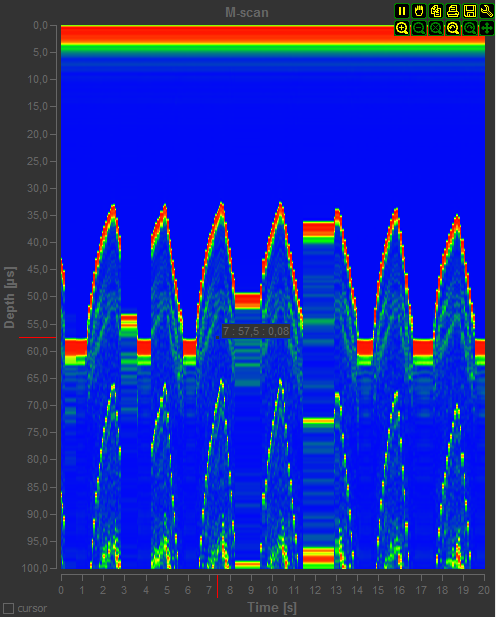
\includegraphics[width=0.6\textwidth]{TimeScan.png}
	\caption{TM-Scan eines pulsierenden Herz-Modells}
	\label{fig:Herz}
\end{figure} \\
Als endsystolisches Herzvolumen ESV bezeichnet man das kleinste Volumen, das während eines Herzzyklus in den Herzkammern ist. Das enddiastolische Volumen EDV dagegen ist das größte Blutvolumen während eines Zyklusses. Das Herzvolumen HZV ist dann definiert als
\begin{align}
	\text{HZV} = (\text{EDV} - \text{ESV}) \cdot \nu \ .
\end{align}